%
% quantenfeldtheorie.tex -- Quantenfeldtheorie:  Quantisierung, Schrödinger-Gleichung, der harmonische Oszillator, Photonen als Oszillatoren
%
% (c) 2020 Prof Dr Andreas Müller, Hochschule Rapperswil
%
% !TEX root = ../../buch.tex
% !TEX encoding = UTF-8
%
\section{Quantenfeldtheorie\label{fourier:section:quantenfeldtheorie}}
\kopfrechts{Quantenfeldtheorie}
Die beiden Wörter Quanten und Quantisierung ähneln sich, ihre Bedeutungen jedoch nicht. 
Ein Quant ist das kleinstmögliche Teilchen, während Quantisierung nichts anderes bedeutet als zählbar machen. 
In der Quantenfeldtheorie ist genau dieser Schritt von zentraler Bedeutung. Dabei werden klassische Felder wie das elektromagnetische Feld in quantenmechanische Operatoren überführt, wodurch die zuvor kontinuierlichen Felder plötzlich aus einzelnen Quanten bestehen.

In der Primarschule wurde uns beigebracht, dass Dinge, die nicht zählbar sind, stets den Artikel ``das'' enthalten. 
Ist es nun ``das Licht'' oder ``die/der'' Licht? 

Im Folgenden ein geschichtlicher Exkurs, wie es dazu kam.




\subsection{Die Idee der Quantisierung\label{fourier:subsection:DieIdeeDerQuantisierung}}
	
	Die beiden Wörter Quanten und Quantisierung ähneln sich, dessen bedeutung jedenfall nicht. Ein Quant ist ein kleinst mögliches Teilchen und Quantisierung bedeutet nichts Anderes als zählbar. In der Quantenfeldtheorie ist Alles Zählbar, auch Licht. In der Primarschule wurde uns gelehrt, dass Dinge die nicht zählbar sind, stets "das" als vording haben. Das Licht ist also offensichtlich inkorrekt. Nun erfolgt ein  Geschichtlicher Exkurs, wie es dazu kam. 
	
	Mit 16 Jahren fragte Max Planck seinen Professor, ob sich ein Studium in der Physik lohne. 
	Dieser antwortete:
	
	\begin{center}
		\textit{"{}In diesem Fach ist im Grunde schon alles entdeckt, was es zu entdecken gibt.\\
			Es bleibt höchstens noch, ein paar Lücken auszufüllen."}
	\end{center}
	
	Das war 1874. 
	Zum Glück liess sich Planck davon nicht abhalten.
	1897 wurde er Professor für Physik und beschäftigte sich mit einem dieser ungelösten Probleme, der Schwarzkörperstrahlung, auch bekannt als die ultraviolette Katastrophe. 
	UV Strahlung umfasst den Wellenbereich von 0.01 $\mu$m bis 0.4 $\mu$m.
	Nach dem Rayleigh-Jeans-Gesetz steigt die abgegebene Strahlung eines Körpers mit der Frequenz immer weiter an. Bei tiefen Frequenzen stimmt das, aber im ultravioletten Bereich versagt die Theorie komplett. 
	Sie sagt unendlich hohe Energien voraus, während in Wirklichkeit kaum noch Strahlung messbar ist.
	Planck suchte drei Jahre lang nach einer Lösung. 
	
	
	Am Ende war es eher ein Akt der Verzweiflung als eine geniale Eingebung. 
	Planck suchte nicht nach einer neuen Theorie, sondern nach einem mathematischen Trick, der zu den Messwerten passte.
	Ohne genau zu verstehen, was seine Formel physikalisch bedeutete, passte er sie so an, dass sie die experimentellen Daten korrekt beschrieb. 


	\begin{equation}
		B(\lambda, T) = \frac{2 \pi h c^2}{\lambda^5} \cdot \frac{1}{e^{\frac{h c}{\lambda k_B T}} - 1}
	\end{equation}
	

	%https://de.wikipedia.org/wiki/Rayleigh-Jeans-Gesetz#/media/Datei:PlanckWienRayleigh_linear_150dpi_de.png

		
	\begin{figure}[htbp]
		\centering
		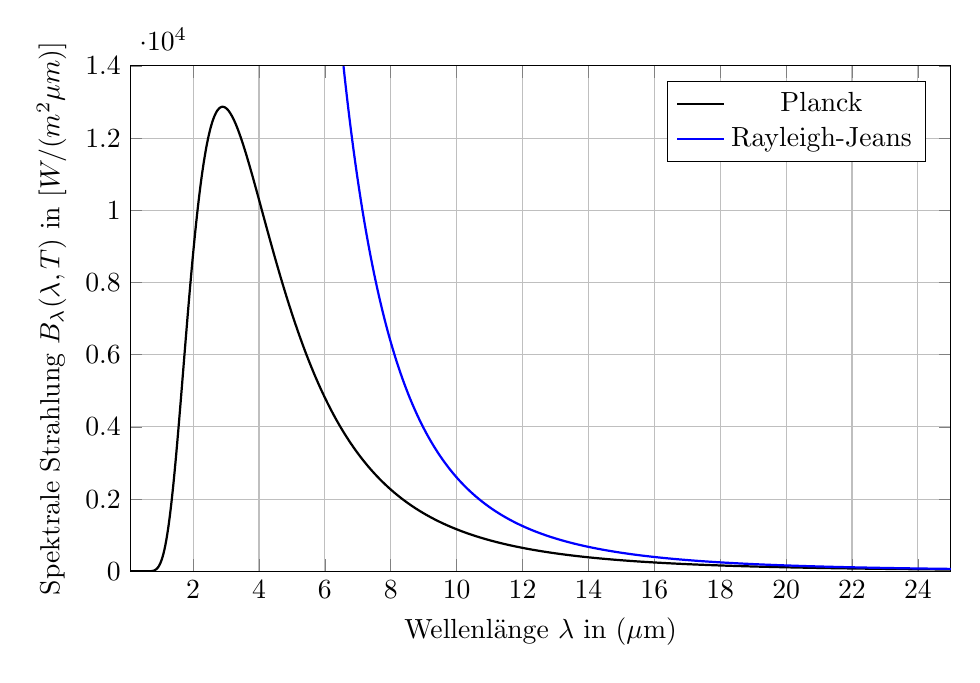
\begin{tikzpicture}
			
			% Hauptachse (linke y-Achse; Werte von 0 bis 14000)
			\begin{axis}[
				name=leftaxis,
				width=12cm,
				height=8cm,
				xlabel={Wellenlänge $\lambda$ in ($\mu$m)},
				ylabel={Spektrale Strahlung $B_\lambda(\lambda, T)$ in $[W/(m^2 \mu m)]$},
				xmin=0.1, xmax=25,
				ymin=0, ymax=14000,
				legend style={at={(0.97,0.97)}, anchor=north east},
				grid=both,
				domain=0.01:26,
				samples=1000
				]
				%W\,m$^{-2}$m$^{-1}
				% Konstanten (SI)
				\def\h{6.62607015e-34}       % Plancksche Konstante
				\def\c{2.99792458e8}         % Lichtgeschwindigkeit
				\def\kB{1.380649e-23}        % Boltzmann-Konstante
				\def\T{1000}                 % Temperatur in Kelvin
				
				% --- Plancksche Strahlungsformel ---
				\addplot[black, thick] 
				expression{
					(2*pi*\h*\c^2)/((x*1e-6)^5) * 1/(exp(\h*\c/((x*1e-6)*\kB*\T)) - 1) / 1e6
				};
				\addlegendentry{Planck}
				
				
				% --- Rayleigh-Jeans-Gesetz (Langwellennähe) ---
				\addplot[blue, thick, restrict y to domain=0:14000]
				expression{
					(2*pi*\c*\kB*\T)/((x*1e-6)^4) / 1e6
				};
				\addlegendentry{Rayleigh-Jeans}
				
				
			\end{axis}
			
			
			
		\end{tikzpicture}
		\caption{Strahlungsspektren nach Planck und Rayleigh-Jeans bei $T=1000\,\mathrm{K}$}
	\end{figure}
		

	



	
	
	
	Früher nahm man an, die Energie einer Welle hänge nur von ihrer Amplitude ab. 
	Man glaubte auch, Atome könnten jede beliebige Energiemenge abstrahlen. Plancks Modell stellte das infrage. 
	Energie konnte nur in bestimmten Portionen abgegeben werden, abhängig von der Frequenz und nicht von der Amplitude.
    Er führte eine neue Naturkonstante ein, das Plancksche Wirkungsquantum $h = 6{,}626 \times 10^{-34} \ \text{J\,s}$. 
	
	
	\begin{equation}
		E = h \cdot f
	\end{equation}
	 
	 
	Je höher die Frequenz, desto grösser ist das nötige Energiepaket. 
	Deshalb nimmt die Strahlung bei hohen Frequenzen wieder ab. Denn hohe Frequenzen bedeuten viel Energie pro Lichtquant und es ist ziemlich unwahrscheinlich, dass ein einzelnes Atom so viel Energie auf einen Schlag abgibt. 
	Planck wusste dies nicht. 
	Aber mit seiner Formel war der erste Schritt in Richtung Quantentheorie gemacht.
	
	%Einstein
	
	
	1905 kam Albert Einstein ins Spiel. 
	Er nahm Plancks Idee und dachte sie weiter. 
	Licht, das man bisher nur als elektromagnetische Welle kannte, sollte sich manchmal wie ein Teilchen verhalten.
	Er nannte diese Teilchen Lichtquanten, heute sagen wir Photonen. 
	Mit dieser Vorstellung konnte er den photoelektrischen Effekt erklären, ein Experiment, das sich mit klassischer Physik nicht deuten liess. 
	Für diese Arbeit bekam er 1921 den Nobelpreis.
	 
	%Bohr
	
	1913 übertrug Niels Bohr die Quantisierung auf Atome. 
	In seinem Modell durften Elektronen nur auf festen Bahnen existieren. 
	Ein Übergang zwischen diesen diskreten Bahnen ging immer mit einer Energieabgabe oder aufnahme in Form eines Photons einher. 

	%de Broglie
	
	Louis de Broglie stellte die Frage, ob Teilchen ebenfalls wellenartige Eigenschaften besitzen könnten. 
	Er postulierte, dass jedes Teilchen mit Impuls $p$ eine Wellenlänge besitzt, die durch
	
	
	\begin{equation}
		\lambda = \frac{h}{p}
	\end{equation}
	
	
	gegeben ist. So verband er die Konzepte von Materie und Welle.
	
	%Schrödinger
	
	Erwin Schrödinger entwickelte schliesslich eine Wellengleichung, die das Verhalten dieser Materiewellen beschreibt. Die eindimensionale zeitabhängige Schrödingergleichung lautet:
	
	
	\begin{equation}
		i \hbar \frac{\partial \psi(x,t)}{\partial t} = -\frac{\hbar^2}{2m} \frac{\partial^2 \psi(x,t)}{\partial x^2} + V(x) \psi(x,t)
	\end{equation}
	
	
	Anstatt exakte Bahnen zu liefern, gibt sie die Wahrscheinlichkeitsverteilung für den Aufenthaltsort eines Teilchens an, ein Grundprinzip der Quantenmechanik.
	
	So wurde klar, dass die Welt im Kleinen ganz eigene Regeln besitzt, die sich mathematisch erfassen lassen.
	
	
	

\subsection{Der harmonische Oszillator\label{fourier:subsection:derHarmonischeOszillator}}
Warum genau schauen wir uns den harmonischen Oszillator an?
In der Quantenelektrodynamik werden die elektromagnetischen Felder als quantisierte harmonische Oszillatoren modelliert, deren Energie ebenfalls in Vielfachen von $\hbar\cdot\omega$ vorliegt.
Die Zustände des Feldes (Photonenzahlenzustände) werden durch die Schwingungszustände des harmonischen Oszillators beschrieben.

Diese Quantisierung erklärt, warum Licht in Lasern nicht kontinuierlich, sondern in diskreten Paketen (Photonen) emittiert wird. % todo: diesen Satz an anderer passenden Stelle einfügen

Die Wellengleichung lautet bekanntlich
\begin{equation}
    \frac{\partial^2 u}{\partial t^2} = c^2 \left( \frac{\partial^2 u}{\partial x^2} + \frac{\partial^2 u}{\partial y^2} \right).
\end{equation}
Wenn nun der y-Anteil als konstant betrachtet wird, sind alle partiellen Ableitungen nach y gleich Null.
Dies führt zu der vereinfachten Gleichung
\begin{equation}
    \frac{\partial^2 u}{\partial t^2} = c^2 \frac{\partial^2 u}{\partial x^2}.
\end{equation}
Daraus lässt sich die Differentialgleichung
\begin{equation}
    \ddot{a}(t) = -k^2 a(t)
\end{equation}
aufstellen.
$a(t)$ ist hierbei ein Fourier-Koeffizient des elektromagnetischen Wellenfeldes.
Die Lösung dieser Differentialgleichung lautet
\begin{equation}
    u(t,x) = a_k(t) \cos(kx)
\end{equation}

% Besser sin verwenden --> besser e^ikx verwenden; Überlegen, ob wir komplex arbeiten möchten
% In Präsentation mit cos und im Paper mit e^ikx


% Wichtiger Schritt: Der harmonische Oszillator in der Quantenmechanik --> Unterlagen anschauen. 
% Evtl. Termin mit ihm, um Unklarheiten zu klären.

% Gutes Video, welches den harmonischen Oszillator erklärt.
%       https://www.youtube.com/watch?v=5P19hROy9vk
% quantenmechanik: Energie ist auch Quantisiert;
% Oszillator kann nur auf bestimmten Leveln schwingen.
% Energielevel haben dieselben Abstände (quadratischer Brunnen)

% further theory: https://www.youtube.com/watch?v=OdizRUe84bg&list=PL8W2boV7eVfmdWs3CsaGfoITHURXvHOGm

Diese Gleichung ist analog zur Gleichung eines Federpendels.
Es handelt sich hier um ein ``Quanten-Federpendel''.    
\begin{figure}
\centering
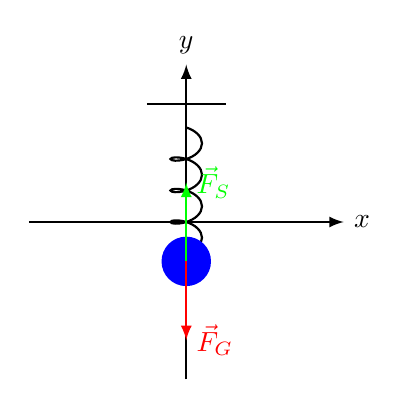
\begin{tikzpicture}[>=latex,thick]
    % Koordinatensystem
    \draw[->] (-2,0) -- (2,0) node[right] {$x$};
    \draw[->] (0,-2) -- (0,2) node[above] {$y$};
    
    % Feder
    \draw[thick] (0,1.5) -- (0,1.2);
    \draw[thick, decorate, decoration={coil, aspect=0.5, segment length=4mm, amplitude=2mm}] (0,1.2) -- (0,-0.5);
    
    % Körper
    \filldraw[blue] (0,-0.5) circle (0.3) node[below] {$m$};
    
    % Kräfte
    \draw[->, thick, red] (0,-0.5) -- (0,-1.5) node[right] {$\vec{F}_G$};
    \draw[->, thick, green] (0,-0.5) -- (0,0.5) node[right] {$\vec{F}_S$};
    
    % Aufhängung
    \draw[thick] (-0.5,1.5) -- (0.5,1.5);
\end{tikzpicture}
\caption{Federpendel}\label{fourier:figure:federpendel}
\end{figure}

%%
\subsection{Einführung in Werkzeuge der Quantenmechanik\label{fourier:subsection:WerkzeugeQuantenmechanik}}
Für die Erklärung von Photonen sind einige Werkzeuge der Quantenmechanik nützlich, welche nachfolgend kurz eingeführt werden.

\subsubsection{Bra-Ket-Notation\label{fourier:subsubsection:BraKetNotation}}
Die Bra-Ket-Notation, auch Dirac Notation genannt, wird in der Quantenmechanik häufig verwendet.
Sie wurde von Paul Dirac eingeführt und ist sehr praktisch, um Zustände und Operatoren kompakt und elegant darzustellen.
\begin{equation}
	\langle \psi | \phi \rangle
\end{equation}
ist eine abgekürzte mathematische Schreibweise für
\begin{equation}
	\int \psi^*(x)\,\psi(x)\,dx
\end{equation}
$\psi$ steht nach wie vor für die Wellenfunktion und wird hier zur Erläuterung der Bra-Ket-Notation verwendet.
Die Bra-Ket-Notation besteht aus zwei Hauptteilen.
Ket $\langle \psi |$ beschreibt einen Zustand beispielsweise eines Systems oder der Wellenfunktion.
Bra $| \phi \rangle$ ist das duale (konjugiert komplexe) zu $\langle \psi |$.
A ist ein Operator (z.B. Hamilton-Operator, Impulsoperator, Ortsoperator).

\subsubsection{Unschärferelation\label{fourier:subsubsection:Unschaerferelation}}
In der Quantenmechanik gibt es keine festen Werte, sondern Wahrscheinlichkeiten und Mittelwerte.
In der klassischen Physik ist es der Impuls p, wohingegen in der Quantenmechanik der Impuls ein Operator 
\begin{equation}
	p - i \, \hbar \frac{d}{dx}
\end{equation}
ist.
Man kann nicht einfach sagen ``Das Teilchen hat einen Impuls p'', weil der Impuls unscharf (nicht exakt bestimmt) sein kann.
Der Ort und der Impuls sind nicht gleichzeitig messbare Observablen.
Ihre Operatoren vertauschen nicht
\begin{equation}
    [\hat{x}, \hat{p}] = i\hbar.
\end{equation}
Aus dieser Vertauschungsrelation folgt mathematisch direkt die Unschärferelation.
Die Unschärferelation ist kein Messfehler, sondern ein fundamentales Naturgesetz.
Diese Relation sagt, dass es eine Grenze gibt, wie präzise man einen Ort und einen Impuls gleichzeitig kennen kann.
Es ist ein Ausdruck der Wellen-Natur von Teilchen.
% todo knma: Ergänzungen anbringen

\subsection{Beweis des Photons\label{fourier:subsection:BeweisPhoton}}
Mit dem Grundwissen, welches in den bisherigen Kapiteln dieses Papers vermittelt wurde und den vorgestellten Werkzeugen der Quantenmechanik wird in diesem Kapitel bewiesen, dass das Photon exisitert.

Die Hamilton-Funktion
\begin{equation}
	H(x,p) = T(p) + V(x)
\end{equation}
ist eine Funktion von Positionen (x) und Impulsen (p).
Sie beschreibt die Gesamtenergie eines Systems.
Dienend als Grundlage für Hamiltonische Gleichungen beschreibt sie die Systembewegung.
%todo: evtl. simpler schreiben.
T (p) ist die kinetische und V (x) ist die potentielle Energie.
%Mit Notizen
% todo: add some stuff of book quantum mechanics to glue things together

Durch Schrödinger wird der Impuls p durch
\begin{equation}
	\frac{\hbar}{i} \frac{\partial}{\partial x}
\end{equation}
ersetzt.
Wodurch
\begin{equation}
	\hat{H} = -\frac{\hbar^2}{2m}\frac{\partial^2}{\partial x^2} + V(x)
\end{equation}	
der Hamiltonoperator resultiert.

% todo: Überleitung
Der Erwartungswert des Impulses
% todo equation
ist der mittlere (erwartete) Impuls, wenn das System im Zustand $| \phi \rangle$ ist.
% todo: somehow from Bra-Ket to measuring values